\documentclass{beamer}
\usetheme{Madrid}

\usepackage{amsmath,amssymb,amsfonts,amsthm}
\usepackage{graphicx}
\usepackage{listings}
\usepackage{gensymb}
\usepackage{xparse}

\usepackage[utf8]{inputenc}
\usepackage{hyperref}
\newcommand{\createMat}[2]{\begin{pmatrix} #1 \\ #2 \end{pmatrix}}

\begin{document}

\title{1.5.16}
\author{ai24btech11035 - V.Preethika}
\date{}
\frame{\titlepage}

\begin{frame}
\frametitle{Question}
Find the coordinates of a point A where AB is a diameter of the circle with center (3, -1) and the point B is (2, 6).\\
\end{frame}

\begin{frame}[allowframebreaks]
\frametitle{Solution}
\begin{table}[htbp]
\centering
  
    \begin{tabular}{ |c|c|c| }
        \hline
	    \textbf{Point} & \textbf{Value} & \textbf{Description}\\ 
        \hline
	    $\text{C}$ & $(3, -1)$ & $\text{Centre of the cicle}$ \\ 
        \hline
	    $\text{B}$ & $(2, 6)$ & $\text{Given point B}$ \\ 
        \hline
	    $\text{A}$ & $(x, y)$ & $\text{Coordinates of A}$ \\ 
        \hline
    \end{tabular}



	\caption{Variables Used}
	\label{tab1.5.16}
\end{table}
	\begin{align}
    \vec{C} &= \frac{\vec{A}+\vec{B}}{2} \\
		&= \frac{\createMat{x}{y} + \createMat{2}{6}}{2} \\
             &= \left(\frac{x+2}{2}, \frac{y+6}{2}\right)
	\end{align}
	  
    
		Given the centre of the circle $\vec{C}$ is (3,-1),we can write
    
		\begin{align}
    \left( \frac{x + 2}{2}, \frac{y + 6}{2} \right) = (3, -1)
		\end{align}
    
    By solving this two equations we get:
    \begin{align}
	    x &= 4 \\
	    y &= -8
    \end{align}

    
    Therefore, the coordinates of point $\vec{A}$ are (4, -8).
\end{frame}
% Define colors for syntax highlighting
\definecolor{codegreen}{rgb}{0,0.6,0}
\definecolor{codegray}{rgb}{0.5,0.5,0.5}
\definecolor{codepurple}{rgb}{0.58,0,0.82}
\definecolor{backcolour}{rgb}{0.95,0.95,0.92}

% Settings for the C code
\lstset{
    language=C,
    basicstyle=\footnotesize\ttfamily,
    backgroundcolor=\color{backcolour},
    commentstyle=\color{codegreen},
    keywordstyle=\color{blue},
    numberstyle=\tiny\color{codegray},
    stringstyle=\color{codepurple},
    breakatwhitespace=false,
    breaklines=true,
    captionpos=b,
    keepspaces=true,
    numbers=left,
    numbersep=5pt,
    showspaces=false,
    showstringspaces=false,
    showtabs=false,
    tabsize=2
}
\begin{frame}[fragile,allowframebreaks]
\frametitle{C Code}
\lstinputlisting[label=mycode1]{codes/data.c}
\end{frame}
% Define colors for syntax highlighting
\definecolor{codegreen}{rgb}{0,0.6,0}
\definecolor{codegray}{rgb}{0.5,0.5,0.5}
\definecolor{codepurple}{rgb}{0.58,0,0.82}
\definecolor{backcolour}{rgb}{0.95,0.95,0.92}

% Python style for highlighting
\lstset{
    language=Python,
    basicstyle=\ttfamily\small,
    keywordstyle=\color{blue},
    stringstyle=\color{codepurple},
    commentstyle=\color{codegreen},
    backgroundcolor=\color{backcolour},
    breaklines=true,
    breakatwhitespace=true,
    tabsize=4
}

\begin{frame}[fragile,allowframebreaks]
\frametitle{Python Code}
\lstinputlisting[label=mycode1]{codes/plot.py}
\end{frame}
\begin{frame}
\frametitle{Plot}
\begin{figure}[htbp]
	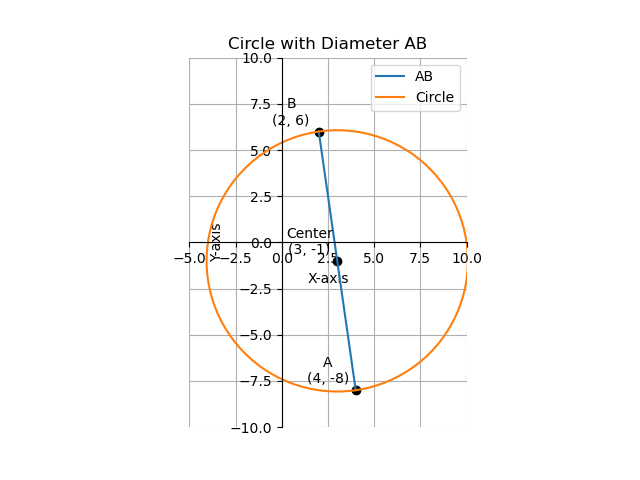
\includegraphics[width=0.75\columnwidth]{figs/plot.png}
	\caption{Plot of $y(x)$}
	\label{fig:bode}
\end{figure}
\end{frame}
\end{document}

